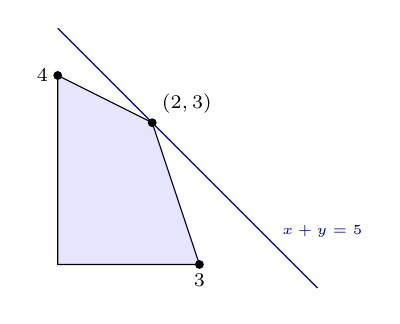
\begin{tikzpicture}[x=6mm,y=6mm]
\fill[blue!10] (0,0)--(3,0)--(2,3)--(0,4)--cycle;
\ax{-1}{6.5}{-1}{6}
\draw[blue!60!black,domain=0:5.5,samples=80] plot (\x,{5-\x});
\fill (2,3) circle (1.6pt);
\node[above right] at (2,3){\scriptsize $(2,3)$};
\fill (3,0) circle (1.6pt);
\node[below] at (3,0){\scriptsize 3};
\fill (0,4) circle (1.6pt);
\node[left] at (0,4){\scriptsize 4};
\draw (0,0)--(3,0)--(2,3)--(0,4)--cycle; \node[blue!60!black] at (5.6,0.7){\tiny $x+y=5$};
\end{tikzpicture}